\documentclass[a4paper]{article}
\usepackage[utf8]{inputenc}
\usepackage[russian]{babel}
\usepackage{listings}
\usepackage[a4paper]{geometry}
\usepackage{indentfirst}
\usepackage{graphicx}
\usepackage{caption}
\usepackage{float}
\usepackage{amssymb}
\usepackage{physics}

\begin{document}

\title{Лабораторная работа 5 по курсу <<Нелинейная динамика и её приложения>>. \\Отчёт.}
\author{Владислав Соврасов\\ 381503м4}
\date{}
\maketitle

\section{Оценка качества нахождения Флоке-базиса для уравнения Шрёдингера c
периодическим по времени гамильтонианом}
Рассматриваается уравнение Шрёдингера с периодической правой частью:
\begin{displaymath}
	i \dot{\ket \psi} = H(t)\ket \psi, H(t)=H_0 + F \sin(\frac{2\pi}{T} t)H_1,
\end{displaymath}
в котором \(H_0, H_1\) --- GUE матрицы.

Для нахождения Флоке-базиса в момент времени \(T\) используется матрица-пропагатор \(U(T)\).
Как было выяснено, её собственные векторы являются Флоке-базисом в моменты \(kT\),
а собственнные значения определяют квазиэнергии системы.

При нахождении каждого из столбцов матрицы \(U(T)\) применялось численное интегрирование
методом Рунге-Кутты из стандартных базисных ортов евклидова пространства.

Если взять в качестве начального условия один из векторов Флоке-базиса и подействовать на
него пропагатором, то \(\ket{\psi(T)}=U(T)\ket{\varphi(0)}=\mu\ket{\varphi(0)}\). Сравнивая это с
теоремой Флоке (\(\ket{\psi(T)}=e^{i\Xi T}\ket{\varphi(T)}\)), получим что, \(\mu=e^{i\Xi T}\); откуда следует, что
в качестве оценки ошибки нахождения собственных числел \(U(T)\) можно рассматривать величину
\(\varepsilon_\mu = \max_{k=\overline{1,N}}||\mu_k|-1|\).

На рис. \ref{fig:eigvals_error} показан график зависимости \(\varepsilon_\mu\) от
шага интегрирования для системы размерности 100 при \(F=0.1,T=1\). Как видно из графика, ошибка при
уменьшении шага убывает с четвёртым порядком.

В качестве оценки ошибки нахождения собственных векторов использовалась величина
\(\varepsilon_\varphi=\max_{k=\overline{1,N}}\Vert U_{\frac{h}{2}}(T)\ket{\varphi_{k,h}} -\mu_{k,h}\ket{\varphi_{k,h}}\Vert\),
где \(h\) --- шаг интегрирования, с которым получены пропагатор и соответствующие векторы и собственные числа.
Фактически, эта запись эквивалентна численному интегрированию системы с половинным шагом
из начальных условий \(\ket{\varphi_{k,h}}\) и последующему сравнению с результатом
пропагации \(U_h(T)\ket{\varphi_{k,h}}=\mu_{k,h}\ket{\varphi_{k,h}}\), полученным с одинарным шагом. На рис. \ref{fig:eigvecs_error}
показана зависимость \(\varepsilon_\varphi\) от шага интегрирования для той же системы размерности
100, что рассматривалась ранее. Величниа \(\varepsilon_\varphi\), как и \(\varepsilon_\mu\),
при уменьшении шага убывает с четвёртым порядком.

\begin{figure}[H]
	\center
	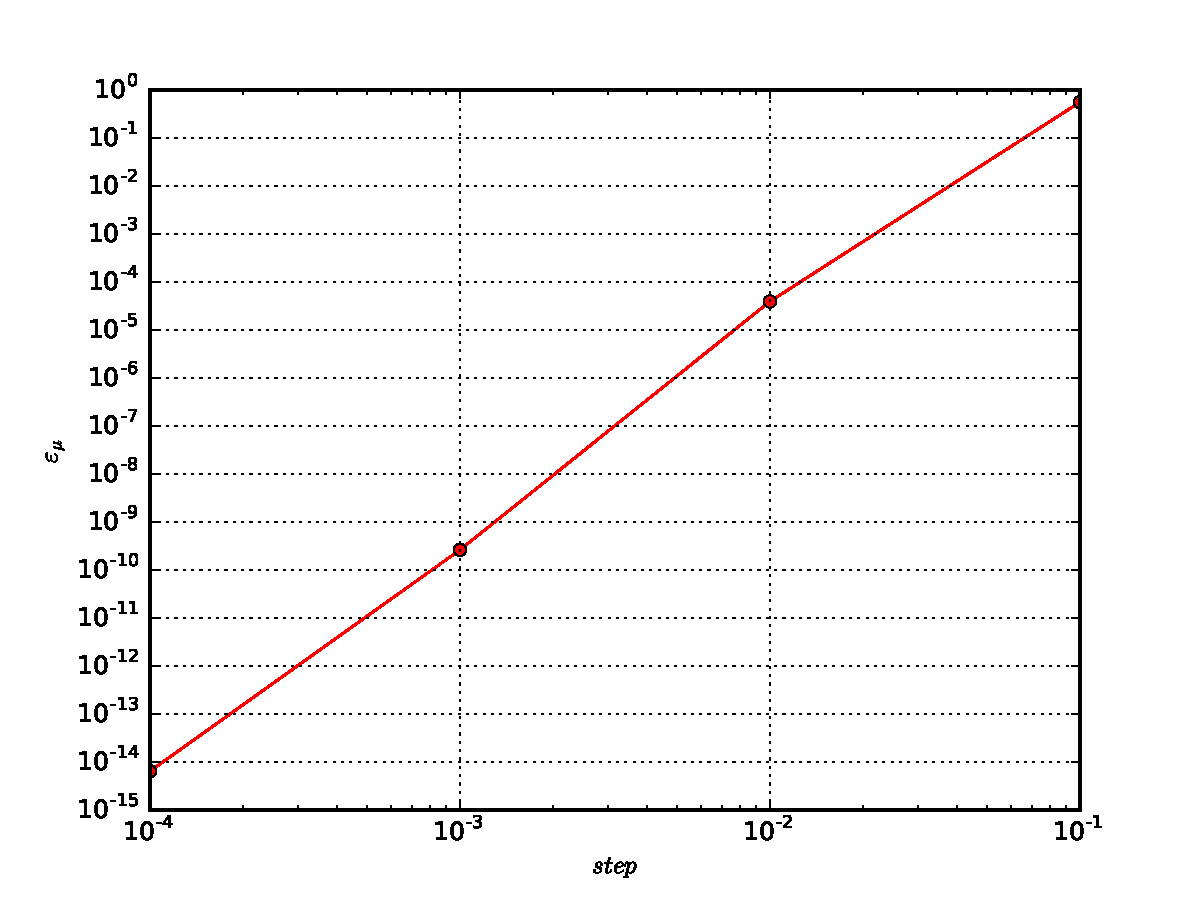
\includegraphics[width=0.75\textwidth]{../pictures/lab5_eigvals_error.pdf}
	\caption{Отклонение модуля собственных чисел матрицы-пропагатора от 1}
	\label{fig:eigvals_error}
\end{figure}

\begin{figure}[H]
	\center
	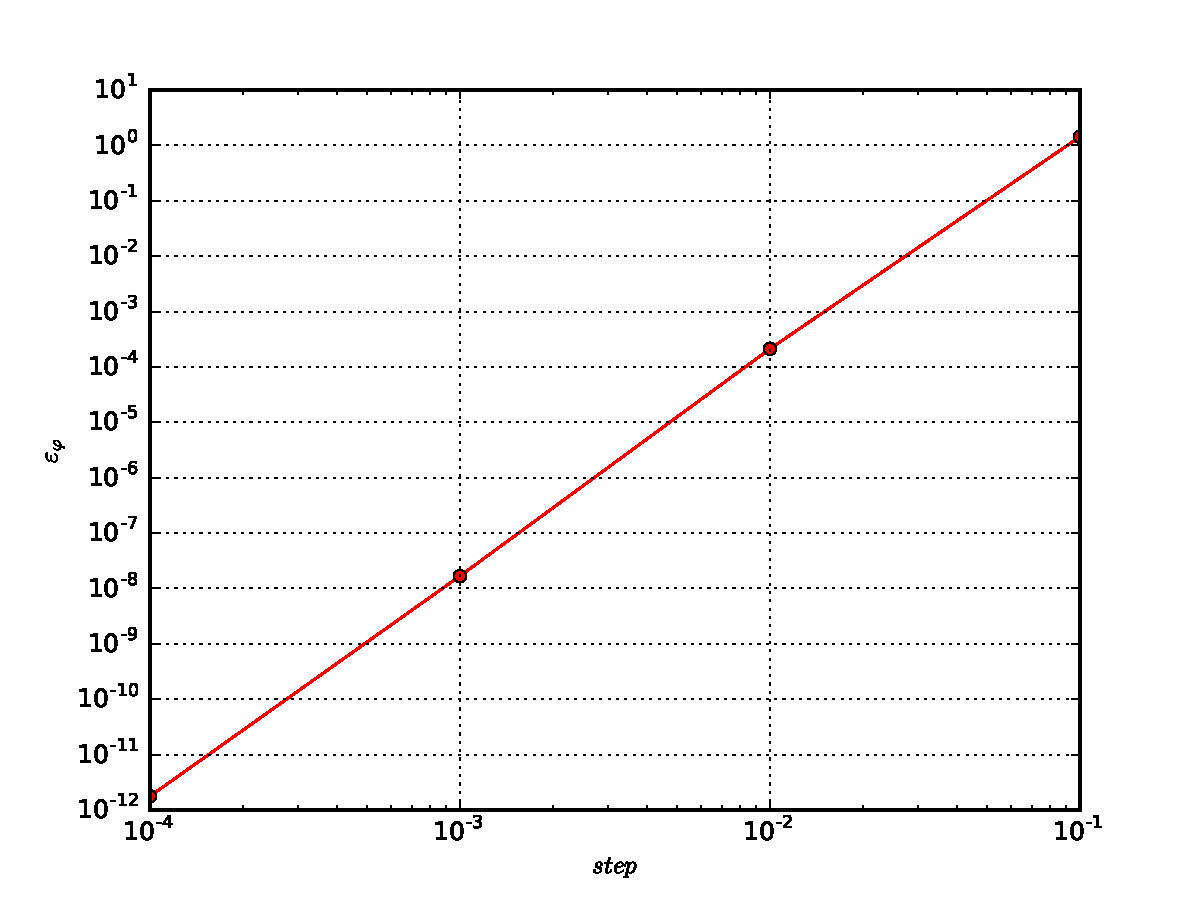
\includegraphics[width=0.75\textwidth]{../pictures/lab5_eigvecs_error.pdf}
	\caption{Оценка ошибки нахождения собственныx векторов матрицы-пропагатора}
	\label{fig:eigvecs_error}
\end{figure}

\section{Исходный код}
\lstinputlisting[language=Python, numbers=left]{../scripts/lab5.py}

\end{document}
